\documentclass[conference]{IEEEtran}
\IEEEoverridecommandlockouts

\usepackage{cite}
\usepackage{amsmath,amssymb}
\usepackage{graphicx}
\usepackage{booktabs}
\usepackage{multirow}
\usepackage{url}
\usepackage[table]{xcolor}
\usepackage[hidelinks]{hyperref}

\newcommand{\best}[1]{\textbf{#1}}
\newcommand{\ours}{\textsc{Reg+Chamfer}}

\begin{document}

\title{CrackID: A Benchmark for Crack Re-Identification,\\
and the Limits of Appearance Matching}

\author{\IEEEauthorblockN{Anonymous Submission}
\IEEEauthorblockA{Paper ID \textemdash{} \textit{under review}}}

\maketitle

\begin{abstract}
Automated maintenance systems turn photographs into tracked defect records, so a
defect re-photographed across visits must be re-identified: the new photo must
match the specific physical crack's record, or open a new one. Despite mature
crack \emph{detection}, we know of no dataset or benchmark for crack
\emph{re-identification}, and the natural approach --- crop the region and match
embeddings --- imports an assumption from person/vehicle re-ID that may not
transfer: that a crack has stable, locally distinctive appearance.
We introduce \textsc{CrackID}: 140 photographs over 17 walls with 212 crack
identities, released with an explicit annotation-quality report and with every
metric's chance level stated. Each wall was captured in one continuous
walk-around, so the benchmark measures \emph{within-visit viewpoint robustness};
a synthetic multi-visit protocol (warp plus grown or corrupted appearance) is
reported as a secondary check, and re-identification across real sessions is a
hypothesis here, not a result. Benchmarking nine matchers across four families, we
find that on the decision a system actually makes --- \emph{same crack or not},
at a threshold --- none exceeds chance by more than $0.054$ pairwise $F_1$,
two achieve nothing, and at a validation-calibrated threshold eight of the nine span only
$-0.012$ to $+0.012$ around chance while LoFTR holds a margin of $0.046$.
These are point estimates on an effective sample of $19$ identities over $11$
walls; the wall-level intervals are wide (Sec.~\ref{sec:validity}), so the
claim is the structure --- a band at the floor with one exception --- not the
individual digits.
Two controls localise the difficulty: giving an embedder the surrounding wall
raises its open-set rate $0.168 \to 0.404$, but \emph{erasing the crack} from
that view costs almost none of it ($0.393$) --- such a method retrieves on
location, not crack appearance. A geometric reference baseline --- register on
wall texture with cracks masked \emph{out}, Chamfer-match projected crack masks
under global assignment --- reaches $\mathrm{DIR}@\mathrm{FAR}{=}0.1$ of
$0.768$ against $0.429$ for the best crop method and $0.000$ for a control that
exploits its coverage without examining a crack, so the open-set gap is
attributable to matching, not partial coverage; like the $F_1$ figures these are
point estimates on the same $19$-identity sample, and the claim is the $0.35$
gap as a structure, not a precise spread (Sec.~\ref{sec:validity}).
This is not yet deployment evidence: the geometric system answers only $48\%$
of pairs, fails categorically on two smooth-plaster walls, and its apparent
within-visit advantage is entangled with homography-based annotation provenance;
that circularity is unresolved rather than removed by the two partial checks. On the
synthetic revisit check, which is the paper's only multi-visit evidence,
OSNet$+$context instead wins ranking and open-set performance; the geometric
advantage therefore should not be read as a demonstrated cross-visit solution.
\end{abstract}

\begin{IEEEkeywords}
crack re-identification, dataset, benchmark, building maintenance, structural
inspection, homography, geometric alignment, annotation quality
\end{IEEEkeywords}

\section{Introduction}

Automated building-maintenance systems convert photographs into tracked defect
records: a re-photographed defect must eventually be \emph{re-identified} --- matched to its
record, or given a new one. This paper first studies within-visit re-identification
under viewpoint change. Wall cracks are a common and difficult case, because
the same crack is re-photographed from different distances, angles and lighting,
and (Sec.~\ref{sec:dataset}) grows.

Crack analysis is a mature \emph{detection} and \emph{segmentation} task, and its
datasets --- CrackSeg9k~\cite{kulkarni2022crackseg9k},
OmniCrack30k~\cite{benz2024omnicrack30k} --- carry no cross-observation identity
labels, because the task they serve needs none. We know of no benchmark for crack
\emph{re-identification}; the natural approach, crop-and-match as in person and
vehicle re-ID~\cite{zhou2019osnet,qian2024reidtrends}, assumes a crack has
stable, locally distinctive appearance, and whether it does has never been
measured. We introduce \textsc{CrackID} --- 140 photographs, 17 walls, 212 crack
identities --- to make that re-identification measurement (Fig.~\ref{fig:ceiling}). Capture is one
continuous walk-around per wall, so what is measured is \emph{within-visit}
viewpoint and scale correspondence --- an upper bound on multi-visit
performance; we add a synthetic revisit protocol as a venue-controlled
secondary check (Sec.~\ref{sec:hybridbench}). That check uses a distinct
\emph{Hybrid} pipeline: it extends the Table~I \ours{} registration baseline
with a skeleton-comparison fallback and per-pair blending, so its reversal is
not a direct contradiction of Table~I.

\smallskip
\noindent\textbf{Appearance buys almost nothing on the decision.} On ranking the
nine matchers separate as expected (Rank-1 $0.352$--$0.654$ against $0.336$
chance); on pairwise $F_1$ --- the \emph{same-crack-or-not} decision a record
makes at a threshold --- all nine land between $0.000$ and $0.054$ above the
$0.305$ floor, two (ORB, DeiT) at exactly zero,
and at a validation-calibrated threshold eight of the nine span only $-0.012$ to $+0.012$
around chance while LoFTR holds a real margin of $0.046$.

\smallskip
\noindent\textbf{Two controls say where the difficulty is not.} Giving an
embedder the surrounding wall raises OSNet's open-set rate $0.168 \to 0.404$;
\emph{erasing the crack} from that view costs almost none of it ($0.393$) ---
such a method retrieves on the wall, and the cue that works, even implicitly, is
\emph{location}.

\smallskip
\noindent\textbf{A geometric baseline makes location explicit.} Registering on
non-crack texture, projecting crack masks into a common frame, and Chamfer-matching
under global assignment reaches $\mathrm{DIR}@\mathrm{FAR}{=}0.1$ of $0.768$
against $0.429$ (best crop) and $0.404$ (best context), answering $48\%$ of
pairs; a \textsc{Coverage-only} control scores $0.000$ on the same metric, so the
open-set gap is matching, not alignment coverage. This is a conditional result,
not a deployment-ready system: two test walls have zero registration success,
and the annotation and baseline both use homography-based alignment.
The resulting geometric advantage is therefore a hypothesis about this benchmark,
not an independently established identity effect.

\smallskip
\noindent\textbf{The revisit check reverses the ranking story.} The real data are
one continuous walk-around per wall, minutes apart, not separate visits. Under
the synthetic warp-plus-appearance protocol, OSNet$+$context beats the hybrid at
R@1 ($0.826/0.671$ versus $0.275/0.274$) and open-set rate
($0.739/0.663$ versus $0.343/0.342$) for growth/appearance change; the hybrid's
small assignment-$F_1$ advantage is not evidence that geometry solves real
multi-visit re-identification.

\smallskip
\noindent\textbf{Contributions:} (i)~\textsc{CrackID} with an explicit
annotation-quality report --- $45\%$ of identities were formed by an automatic
merge, reported rather than assumed (Sec.~\ref{sec:annotation}); (ii)~a
nine-method benchmark against stated chance levels, with crop$+$context and
crack-erased controls (Sec.~\ref{sec:ceiling}); (iii)~a synthetic revisit protocol isolating appearance change from damage
evolution --- the only multi-visit evidence this paper has
(Sec.~\ref{sec:hybridbench});
(iv)~a geometric reference
baseline and a protocol for this task's failure modes --- coverage-aware
metrics, unanswerable queries, an admission gate, wall-resampled confidence
(Sec.~\ref{sec:method}, \ref{sec:protocol},~\ref{sec:results}).

\begin{figure}[t]
\centering
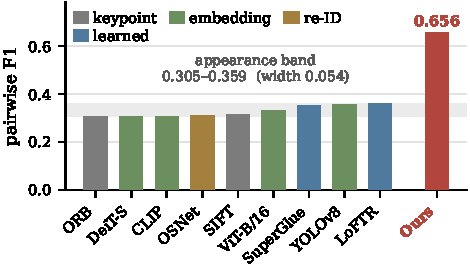
\includegraphics[width=\columnwidth]{figs/ceiling.pdf}
\caption{\textbf{The appearance ceiling.} Pairwise $F_1$ for nine crop-scope
matchers spanning four method families on \textsc{CrackID} test. Every method
falls inside the band $0.305$--$0.359$ --- width $0.054$ --- pressed against the
$0.305$ chance floor ($2p/(1+p)$ for this pool), irrespective of family, era, or
compute budget. The geometric reference baseline (red) leaves the band. Ranking
metrics separate the same methods over a $0.30$ range; the decision metric does
not.}
\label{fig:ceiling}
\end{figure}
\section{Related Work}

Crack analysis is overwhelmingly detection and
segmentation~\cite{hasan2025review,perez2024assessment}; its datasets annotate
cracks within single images and the large consolidations
merging~\cite{kulkarni2022crackseg9k,benz2024omnicrack30k} inherit that scope,
and multi-view pipelines~\cite{mallios2023multiview} aggregate within one
inspection without instance correspondence. Structural-health monitoring does
compare cracks across time with machinery close to
ours~\cite{parente2022monitoring,harb2025multitemporal,sun2025perspective,nec2019guide},
but identity is always \emph{given by construction} (fixed camera, marked
location, operator at a viewpoint): the subject is one known crack, the question
width or extent, and no dataset supports method comparison on the association
decision itself.

Object re-identification~\cite{qian2024reidtrends} with open-set
identification~\cite{liao2014openset} is the formal setting we adopt; keypoint
matching~\cite{lowe2004sift,rublee2011orb}, learned correspondence
(SuperGlue~\cite{sarlin2020superglue}, LoFTR~\cite{sun2021loftr}), and region
embeddings~\cite{dosovitskiy2021vit,touvron2021deit,radford2021clip,zhou2019osnet,oquab2024dinov2}
apply directly to crack crops and our benchmark measures all of them.
Vehicle-damage assessment already re-identifies damage with OSNet in curated
settings~\cite{maiano2023antifraud}; our results suggest the crop scope is
itself the limiting choice. The move our baseline makes --- align two captures,
then reason about what is present in one and absent in the other --- is change
detection~\cite{sakurada2015changedetection,alcantarilla2018street}; planar
registration is classical~\cite{hartley2004mvg,fischler1987ransac,barath2019magsac}
with photometric alignment (ECC~\cite{evangelidis2008ecc}) as the fallback. Our
contribution is not a new estimator but the observation that the alignment
target and the matching target should be \emph{disjoint}: the homography is
driven by the wall precisely because the crack is what we seek to identify.
\section{CrackID}
\label{sec:dataset}

\subsection{Capture and composition}
We photographed 17 exterior walls at one site over four half-days with two
consumer handsets, yielding 140 photographs at $4080\times3072$. The walls span
two surface families that behave very differently under keypoint matching:
stippled render (densely textured) and smooth painted plaster, where the crack is
frequently the only structure in frame. Walls split disjointly into 6 validation
walls (66 photographs, 66 identities) and 11 test walls (74 photographs, 146
identities). Statistical power is governed by identities visible in two or more
photographs --- only these form a query with an answer: 18 in validation, 19 in
test. Each wall was captured in one continuous walk-around (consecutive frames a
median of $3$\,s apart), so the dataset measures \textbf{viewpoint and scale
correspondence} within one visit --- an upper bound on multi-visit performance,
not yet a measurement of it.

\smallskip
\noindent\textbf{The adjacent frame is always an answer.} For $100\%$ of the
$280$ answerable test queries the nearest correct gallery entry is the adjacent
frame. Ranking numbers are therefore near-duplicate retrieval;
Sec.~\ref{sec:results} sweeps the exclusion gap to show the structure is not what
produces the result.

\subsection{Annotation, and why it needs auditing}
\label{sec:annotation}
One click point per crack is propagated across consecutive photographs through an
ORB homography and one-to-one assignment; identities whose components appear to
be fragments of one physical crack are then merged. The merge is where risk
concentrates: a wrongly joined merge converts a hard negative into a free
positive and inflates \emph{every} method's mAP together, so it cannot be caught
by comparing methods. We therefore report its extent rather than assume its
correctness: \textbf{$95/212$ identities ($45\%$) were formed by a merge} (48\%
on test), bridging a median maximum gap of $228$\,px; the adjusted Rand index
against the pre-merge labelling is $0.080$ --- the merge restructured the
partition rather than refining it. We release the instrumentation for an audited
error rate (per-identity provenance, a stratified sample with contact sheets,
Wilson scoring) rather than the audit itself; the verdicts are not yet filled in,
so we claim no sampled error rate.
\section{Benchmark Protocol}
\label{sec:protocol}

A query is one annotated crack instance in one photograph; the gallery is the
query's own wall, so hard negatives share material and lighting; the query's own
photograph and week are excluded, leaving $n_Q = 280$ scored queries on test.
Three choices deliberately favour no method, including ours:
\begin{itemize}\setlength{\itemsep}{1pt}\setlength{\parskip}{0pt}
\item \textbf{Unanswerable queries are retained.} A query whose identity has no
gallery counterpart can contribute false alarms and never successes --- exactly
the open-set case a maintenance system faces.
\item \textbf{Thresholds are calibrated on validation.} Every method reports an
oracle-thresholded $F_1^{*}$ (generous to all) and a deployable $F_1^{@v}$
thresholded on held-out walls.
\item \textbf{Missing scores are charged, not skipped.} A pair a method cannot
score counts as predicted-negative and ranks last; coverage is not independent
of the label (Sec.~\ref{sec:coverage}).
\end{itemize}

\subsection{Metrics}
We report Rank-1, Rank-5 and mAP, pairwise $F_1$, and assignment $F_1$ (a
one-to-one matching per image pair, the deployed operation). The headline metric
is the open-set \textbf{detection-and-identification rate at $10\%$ false alarm}
($\mathrm{DIR}@\mathrm{FAR}{=}0.1$): a known query is correct only if its
top-ranked match is above threshold and correct; an unknown query is a false
alarm whenever anything clears threshold.

\textbf{Every metric is reported against its chance level}, because two are far
from zero: pairwise $F_1$ has a best-constant-predictor floor
$2p/(1+p) = 0.305$ on this
pool, and Rank-5 chance is $0.767$; Rank-1 and $\mathrm{DIR}@\mathrm{FAR}$ chance
are $0.336$ and $0.038$ (closed form, plus $200$ random matrices through the same
evaluation code). This is a prevalence-induced floor, not a coin-flip chance
rate, and it changes when the evaluated pair pool changes. Confidence resamples
\textbf{walls}, not queries --- queries
from one wall succeed or fail together --- and with 11 test walls the interval is
wide; we report its width as the honest statement.
\section{The Appearance Ceiling}
\label{sec:ceiling}

\begin{table*}[t]
\centering
%    10 or 12-token rows ... The prefixed comment must stay stable.
% (see verify_claims.py parse_results_table strictness notes)
\caption{\textbf{Main result}, test split, $n_Q = 280$ query instances over 11
walls. All methods see identical inputs and are scored by identical code.
$F_1^{*}$ is oracle-thresholded on test; $\Delta F_1^{*}$ is its excess over the
$0.305$ best-constant-predictor floor ($2p/(1+p)$, not coin-flip chance;
Sec.~\ref{sec:protocol}); $F_1^{@v}$ is
thresholded on the held-out validation walls and is the deployable number.
\emph{scored} is the fraction of valid query--gallery pairs receiving a finite
score; unscored pairs are charged as predicted-negative and the query is still
counted (Sec.~\ref{sec:coverage}). Cost is wall-clock seconds per query. The
\textsc{Coverage-only} reference row answers yes to every registered pair
without examining a crack and is the level every other row must be read against;
chance levels for every column are given in Sec.~\ref{sec:protocol}. Best
crop-scope value per column in \textbf{bold}.}
\label{tab:main}
\small
\begin{tabular}{llcccccccr}
\toprule
Method & Family & R@1 & mAP & DIR@FAR$=$0.1 & $F_1^{*}$ & $\Delta F_1^{*}$ & $F_1^{@v}$ & scored & s/query \\
\midrule
\rowcolor{black!8}
\multicolumn{10}{l}{\emph{Reference level}} \\
\rowcolor{black!8}
\textsc{Coverage-only} & geometry      & 0.515 & 0.533 & 0.000 & 0.544 & 0.239 & 0.544 & 0.48 & --- \\
\midrule
\multicolumn{10}{l}{\emph{Crop scope}} \\
ORB~\cite{rublee2011orb}            & keypoint   & 0.352 & 0.364 & 0.018 & 0.305 & 0.000 & 0.305 & 1.00 & \best{0.038} \\
SIFT~\cite{lowe2004sift}            & keypoint   & 0.432 & 0.417 & 0.036 & 0.313 & 0.008 & 0.305 & 1.00 & 0.086 \\
SuperGlue~\cite{sarlin2020superglue}& learned    & 0.562 & 0.455 & \best{0.429} & 0.353 & 0.048 & 0.305 & 1.00 & 5.826 \\
LoFTR~\cite{sun2021loftr}           & learned    & 0.549 & 0.440 & 0.336 & \best{0.359} & \best{0.054} & \best{0.351} & 1.00 & 8.639 \\
YOLOv8 backbone                     & embedding  & 0.561 & 0.453 & 0.157 & 0.357 & 0.052 & 0.308 & 1.00 & 0.217 \\
ViT-B/16~\cite{dosovitskiy2021vit}  & embedding  & \best{0.654} & 0.511 & 0.286 & 0.331 & 0.026 & 0.317 & 1.00 & 0.193 \\
DeiT-S~\cite{touvron2021deit}       & embedding  & 0.621 & 0.497 & 0.250 & 0.305 & 0.000 & 0.293 & 1.00 & 0.058 \\
CLIP ViT-B/32~\cite{radford2021clip}& embedding  & 0.604 & 0.471 & 0.143 & 0.307 & 0.002 & 0.306 & 1.00 & 0.050 \\
OSNet~\cite{zhou2019osnet}          & re-ID      & \best{0.654} & \best{0.520} & 0.168 & 0.309 & 0.004 & 0.309 & 1.00 & 0.053 \\
\midrule
\rowcolor{black!5}
\multicolumn{10}{l}{\emph{Full-image scope}} \\
\rowcolor{black!5}
\ours{} (ours) & geometry & \best{0.952} & \best{0.886} & \best{0.768} & \best{0.656} & 0.351 & 0.582 & 0.48 & 27.92 \\
\bottomrule
\end{tabular}
\end{table*}

\subsection{Setup}
Nine crop-scope matchers --- handcrafted keypoints
(SIFT~\cite{lowe2004sift}, ORB~\cite{rublee2011orb}); learned correspondence
(SuperGlue~\cite{sarlin2020superglue}, LoFTR~\cite{sun2021loftr}); general
embeddings (ViT-B/16~\cite{dosovitskiy2021vit}, DeiT-S~\cite{touvron2021deit},
CLIP ViT-B/32~\cite{radford2021clip}, YOLOv8); a re-identification architecture
(OSNet~\cite{zhou2019osnet}) --- run under an identical protocol, inputs and
scoring.

\subsection{Result: appearance buys almost nothing on the decision}
On the decision a record actually makes --- \emph{same crack or not}, at a
threshold --- no crop method clears chance by more than $0.054$ (excess over the
$0.305$ floor at the oracle threshold, Table~\ref{tab:main}: $0.000$--$0.054$,
two methods exactly at the floor, eight within $0.052$), across two decades of
methods and two orders of compute ($\approx\!1$\,ms to $8.6$\,s). At a deployable (validation-calibrated)
threshold eight of the nine span only $-0.012$ to $+0.012$ around chance;
\textbf{LoFTR is the exception}, $F_1^{@v}=0.351$ ($+0.046$), and the most
expensive crop method. Ranking does not transfer to deciding: the nine separate
over a $0.302$ range on Rank-1, yet OSNet ties for best Rank-1 ($0.654$) while
sitting $0.004$ above chance, and SuperGlue (fifth on Rank-1) has the best crop
open-set rate ($0.429$). Ordering a gallery well and keeping a record are not
the same capability. The collapse after validation calibration is consistent
with threshold instability under a small, wall-clustered sample: methods can
order candidates differently while their score distributions do not support a
stable same-crack/not-same-crack boundary on held-out walls. This is an
interpretation of the observed pattern, not a claim that calibration itself is
the sole cause.

\subsection{Is it the crack, or the wall behind it?}
\label{sec:controls}
Two controls separate identity cue from field of view: a \emph{crop$+$context}
condition (wider crop) and a \emph{crack-erased} condition (the crack inpainted
out of that widened view). Context helps a lot --- OSNet's Rank-1 rises
$0.654 \to 0.775$, mAP to $0.595$, open-set rate $0.168 \to 0.404$ (CLIP's
$0.143 \to 0.311$; $F_1^{*}$ $0.309 \to 0.354$) --- \textbf{but erasing the
crack costs almost none of it}: OSNet retains Rank-1 $0.711$, mAP $0.574$ and
open-set $0.393$; CLIP retains Rank-1 $0.600$, mAP $0.502$, open-set $0.286$.
Both erased views still outrank every tight-crop method: the retrieved cue is
the wall, i.e.\ location. Pairwise $F_1$ is unmoved by context
($0.346$--$0.361$). We read the aggregate as a property of the data --- methods
with no shared inductive bias land near the floor, and wherever a crop method
improves, the
improvement is not the crack. Nine methods are a sample, not proof; the result
establishes that the obvious moves buy $0.000$--$0.054$ above chance on the
decision --- reason to change the formulation, not the encoder.
\section{A Geometric Reference Baseline}
\label{sec:method}

The ceiling motivates a change of scope. A crack is a mark at a fixed location
on a rigid, near-planar surface that carries texture the crack does not; we
identify a crack by \emph{where it is on its wall} once the two photographs are
aligned. We release this as a deliberately simple \emph{reference baseline} for
\textsc{CrackID}, with no learned component beyond the shared crack segmenter.

\subsection{Alignment driven by non-crack texture}
A wall is planar, so the homography $x' \sim Hx$ mapping photograph $I_a$ into
$I_b$'s frame is the correct model. The design decision that matters is
\textbf{what drives the fit}: we dilate the crack masks by $15$\,px and exclude
those pixels from detection, so $H$ comes from wall texture alone. This is not an
optimisation but what makes the projected position an independent identity cue ---
were cracks to participate, a long crack could dominate the correspondence set
and pull the fit toward the wrong crack. Detection runs on copies downscaled to
$1600$\,px under CLAHE equalisation; we use SIFT (up to $8000$ features), a
$0.75$ ratio test, and MAGSAC at $4$\,px requiring $25$ inliers.

\subsection{A cascade for two surface families}
One front end does not serve both surfaces, and the failure is categorical: on
the smooth-plaster walls, crack-masked SIFT succeeds on \emph{exactly zero}
pairs. We try three in order: (i)~\textbf{SIFT on masked wall texture}, for
stippled render; (ii)~\textbf{SIFT with cracks restored}, triggered only when
masking starves detection below $300$ keypoints (on plaster the crack is the only
feature in frame), accepting the circularity stage~(i) avoids, and recording
which front end produced each result; (iii)~\textbf{ECC}, direct photometric
alignment over a $320 \to 640 \to 1280$\,px pyramid, on the large-scale shading
that survives on flat paint. Every candidate $H$ is sanity-checked (reject
mirrored/folded quadrilaterals, area scale outside $[1/16,16]$, collapsed sides);
its inlier RMS sets downstream tolerances.

\subsection{Projection and Chamfer agreement}
Crack instances are connected components; pixels from $I_a$ are projected by $H$
and compared with instances of $I_b$. Chamfer distance, not IoU, is the
criterion: cracks are a few pixels wide, so a $3$\,px registration error drives
IoU to zero for a correctly aligned pair. The reported score is the
\textbf{symmetric mean Chamfer distance} in pixels
\begin{equation}
D(a,b) = \tfrac{1}{2}\!\left[
\frac{1}{|a|}\sum_{p \in a} d(p, b) \;+\;
\frac{1}{|b|}\sum_{q \in b} d(q, a)\right],
\label{eq:chamfer}
\end{equation}
over the union bounding box, with cheap rejection when boxes are far apart. We
also report a scale-free alternative --- \textbf{Chamfer coverage}, the symmetric
fraction of pixels within $\tau$ --- because Eq.~(\ref{eq:chamfer}) is a per-pair
pixel distance whose scale differs per pair, so a single global threshold makes
ranking partly measure calibration (Sec.~\ref{sec:chamferablation}).

\subsection{Explicit non-answers, and the licensed negative}
Correspondence is a one-to-one assignment per image pair with an explicit
rejection threshold, not a per-query argmax --- two cracks must not both claim
the same crack; unmatched instances are reported as \emph{disappeared} or
\emph{newly appeared}. The Hungarian solve is part of \emph{evaluation}, applied
identically to every method's score matrix. Specific to this formulation is the
evidence a \textbf{licensed negative} can carry: with $I_a$ projected into
$I_b$'s frame, the system observes a region visible and empty of the recorded
crack --- positive evidence of absence, categorically stronger than the low
similarity a crop embedding produces. A projected crack falling outside the
gallery photograph is a confident rejection, counted separately from unscorable
pairs; this is the mechanism behind the open-set gap
(Sec.~\ref{sec:coverage}).
\section{Results}
\label{sec:results}

\subsection{Main comparison and the open-set gap}
Relocating identity into the wall raises every metric: Rank-1 $0.654 \to 0.952$,
mAP $0.520 \to 0.886$, and as excess over the \textsc{Coverage-only} reference
the ranking gains are $+0.437$/$+0.353$, while pairwise $F_1^{*} = 0.656$ is
$+0.112$ over $0.544$, not the $+0.351$ a comparison against the crop floor would
suggest. The \textbf{open-set result is the one number coverage does not
explain}: $\mathrm{DIR}@\mathrm{FAR}{=}0.1$ reaches $0.768$ against $0.429$ for
the best crop method (SuperGlue), $0.404$ for the best context control, $0.038$
for chance, and exactly $\mathbf{0.000}$ for \textsc{Coverage-only}. Crop methods
cannot decline --- they return a similarity to the nearest neighbour, which on
self-similar hairline cracks is often high --- while an aligned pair supports the
\emph{licensed negative}: the query projects into the gallery frame, where its
region is visible and empty. Compute does not explain the gap: SuperGlue's
$0.429$ costs $5.8$\,s/query, OSNet's $0.168$ costs $0.053$\,s.

\subsection{Partial coverage, gap structure, and failures}
\label{sec:coverage}
Every crop method scores $100\%$ of valid pairs, the geometric method $48\%$;
unscorable pairs are charged as predicted negatives. For \textbf{ranking} that is
a penalty: censoring a complete matrix drops Rank-1 $0.422 \to 0.27$ at $34\%$
coverage. For \textbf{pairwise $F_1$} it is a subsidy: the scorable subset
retains $100\%$ of positives and $36.8\%$ of negatives, so prevalence rises
$0.180 \to 0.373$ and the floor with it, $0.305 \to 0.544$ ---
\textsc{Coverage-only} scores $0.544$ pairwise, mAP $0.533$, Rank-1 $0.515$, above
OSNet, by answering every registered pair without examining a crack. Much of the
ranking and pairwise-$F_1$ margin is therefore \emph{which pairs align}; the
open-set metric is the exception and the result we lead with.

Excluding the adjacent frame, then the two and three nearest, leaves Rank-1 flat
(OSNet $0.654 \to 0.648$) with excess over chance stable in $0.24$--$0.32$: the
near-duplicate structure is real but not what produces the numbers. It is also
important for interpretation: the adjacent frame answers all $280$ queries,
whereas the gap-3 sweep leaves only $105$ answerable queries, so the headline
ranking measures short-baseline correspondence rather than broad temporal
re-identification. Registration
success is strongly wall-dependent ($97/301$ pairs, $32.2\%$: walls 07/08/12
$100\%$, wall 09 $52\%$, wall 11 $83\%$, walls 13--16 between $3\%$ and $29\%$,
walls 10/17 at $0\%$). A logistic fit over all $301$ pairs makes the mechanism
plain: sharpness dominates (median $133.8$ registered vs $7.2$ failed;
wall-clustered Wald $z = 5.1$, $p = 3\times10^{-7}$), frame gap far less
($z = -2.8$, $p = 0.005$). The independent-pairs $z$s ($8.2$, $-5.0$) overstate
the contrast because failure is categorical by wall, so we resample walls, not
queries --- and the leave-one-wall-out spread in Rank-1 is large, so no fine
ranking among baselines is claimed. One admission gate (variance-of-Laplacian
$\geq 10$) applied identically rejects $21$ of $74$ test captures and nearly
doubles registration, $32.2\% \to 56.1\%$.

\subsection{Ablations and cost}
\label{sec:chamferablation}
\textbf{Chamfer distance versus coverage.} The scale-free coverage score
motivated in Sec.~\ref{sec:method} is not a free improvement: it drops mAP
$0.886 \to 0.646$ and Rank-1 $0.952 \to 0.849$, the largest movement any change
produces; $\mathrm{DIR}$ and $F_1^{@v}$ barely move --- coverage gives a threshold
decision, not a ranking. \textbf{Masking.} Disabling crack exclusion leaves
ranking and pairwise agreement practically unchanged (to three decimals) but
raises $\mathrm{DIR}@\mathrm{FAR}$ $0.768 \to 0.825$: masking is not what buys
the reported accuracy. This is expected when the test set contains no deliberate
case where crack pixels create a spurious registration: masking buys evidence
independence, not observed accuracy on this collection, and should be treated as
a safeguard awaiting a harder stress test. \textbf{ECC.} \label{sec:ecc} Disabling
ECC (repaired after a pipeline bug silently left it inert) gives Rank-1 $0.920$,
mAP $0.862$, coverage $0.50$ against $0.952$, $0.886$, $0.48$; assignment $F_1$
rises $0.769 \to 0.784$ when enabled; open-set is unchanged.

\textbf{Cost.} The abstract's more-than-two-orders-of-magnitude comparison at
$27.9$\,s/query is a query-level charging convention, not a fundamental
pair-level compute gap. At $27.9$\,s/query the baseline charges more than two orders of
magnitude above OSNet, but that per-query figure is a charging convention, not
an intrinsic one: registration is per image \emph{pair} --- one homography
serves every crack on a wall --- and amortised over the $301$ test image pairs
the same pass runs $\approx 26$\,s/pair ($7817$\,s total), after which any
later crack query on the pair pays only the Chamfer pass, not the homography.
That pair-level cost is within an order of magnitude of LoFTR ($8.3$\,s), a
crop method with none of the open-set benefit.

\subsection{A synthetic revisit protocol}
\label{sec:hybridbench}
The maintenance setting these records serve is a \emph{revisited} crack, so we
add a second protocol isolating controlled change. Ten source photographs across
five of the walls (walls 01, 02, 04, 05, 09; one seed, $0$) are each synthesized
into a set of queries under an identical warp ($1.08\times$ scale, $6^{\circ}$
rotation, $4^{\circ}$ tilt): dataset A additionally grows every crack tip (damage
evolution), dataset B corrupts appearance while leaving structure untouched
(blur $\sigma{=}1.6$, noise $\sigma{=}14$, brightness/contrast shift); each
synthetic query is ranked against the wall's real instances only. The
\emph{hybrid} folds a structural skeleton comparison into the geometric
baseline as a fallback plus per-pair blend, scored by the same code as
OSNet$+$ctx (Table~\ref{tab:hybrid}).

\begin{table}[t]
\centering
\small
\resizebox{\columnwidth}{!}{%
\begin{tabular}{llccccccc}
\toprule
Protocol & Method & $n_q$ & R@1 & mAP & $\mathrm{DIR}@\mathrm{FAR}{=}0.1$ & $F_1^{@v}$ & $F_1^{a}$ & scored \\
\midrule
A (growth)      & Hybrid      & 69 & 0.275 & 0.401 & 0.343      & 0.569 & 0.646 & 1.00 \\
A (growth)      & OSNet$+$ctx & 69 & \textbf{0.826} & \textbf{0.647} & \textbf{0.739} & 0.601 & 0.631 & 1.00 \\
B (appearance)  & Hybrid      & 82 & 0.274 & 0.403 & 0.342      & 0.574 & 0.640 & 1.00 \\
B (appearance)  & OSNet$+$ctx & 82 & \textbf{0.671} & \textbf{0.570} & \textbf{0.663} & 0.594 & 0.609 & 1.00 \\
\bottomrule
\end{tabular}%
}
\caption{Hybrid versus the strongest appearance baseline on the synthetic
revisit protocol (Sec.~\ref{sec:hybridbench}); pairwise and assignment $F_1$ at
the validation-calibrated threshold. One seed ($0$), ten source photographs
across five walls, no resampling --- rows carry no uncertainty and are an
accuracy checkpoint, not a stability claim (Sec.~\ref{sec:hybridbench}).}
\label{tab:hybrid}
\end{table}

The geometric side does not transfer its main-benchmark advantage here:
OSNet$+$ctx separates the synthetic queries at R@1 $0.826/0.671$, the hybrid at
$0.275/0.274$, with open-set rates $0.739/0.663$ against $0.343/0.342$. But the
split is metric-dependent and opposite the ranking gap: on identity agreement the
hybrid holds its own --- assignment $F_1^{a} = 0.646/0.640$ beats OSNet's
$0.631/0.609$, and pairwise $F_1^{@v} = 0.569/0.574$ trails
$0.601/0.594$ by far less than the ranking margin. Both rate $1.00$ scored, and per cell none was
decided by the pure-homography branch alone ($H\% = 0.0$ --- the share of
assignment cells whose verdict came straight from the homography, with no blend
or skeleton fallback): the geometric pipeline answers
\emph{which crack is which} on pairs appearance also resolves, but loses the
global ranking of a hundred-plus same-wall candidates at one threshold. These
rows are a checkpoint, not a claim: one seed, one wall subset.
\section{Threats to Validity}
\label{sec:validity}

We state the limits in the body because they bound the central claims.

\smallskip
\noindent\textbf{The effective sample is 19 identities.} The test split's $280$
queries come from $19$ identities visible in two or more photographs across $11$
walls; queries from one wall share material, illumination and one camera pass, so
query count is not sample size. We resample walls and report the
leave-one-wall-out spread in Rank-1. The same resampling discipline applies to
the open-set headline: $\mathrm{DIR}@\mathrm{FAR}{=}0.1$ of $0.768$ is a point
estimate at one operating point on the same sample, so the abstract compares it
to baselines as a one-number structure --- the $0.35$ gap --- and claims
nothing about the precise spread between resampled walls. This benchmark supports
a structural claim about the formulation, but not fine-grained ranking among
baselines. We do not attach a numeric wall-resampled interval to the abstract
point estimates because the score matrices needed to recompute it are not part
of the released artefacts; the effective sample and wall-level bimodality should
therefore be read as a limitation, not as hidden precision.

\smallskip
\noindent\textbf{Scope is controlled, and the control found something.} The
method reads full photographs; the baselines read crops --- dictated by design,
since homography needs wall context. Two controls
(Sec.~\ref{sec:controls}) separate identity cue from field of view, and scope
does not account for the open-set gap ($0.404$ best context against $0.768$).
But the crack-erased control is uncomfortable: inpainting the crack costs only
$0.011$ of that $0.404$, so a context-scope number is partly background-matching,
which we expect to weaken on real revisits. Ranking numbers are additionally
near-duplicate (the adjacent frame answers all $280$ queries,
Sec.~\ref{sec:dataset}); the gap sweep shows the trend is flat, with power
falling to $105$ answerable queries by gap $3$.

\smallskip
\noindent\textbf{The annotation and baseline are circularly coupled.}
Identities were seeded by propagating one click point between consecutive
photographs through an ORB homography (Sec.~\ref{sec:annotation}), and the
geometric baseline's whole mechanism is homography registration. Of the $118$
positive (same-crack) query--gallery pairs on test, $116$ ($98.3\%$) involve an
identity formed by a merge; both-sides-unmerged positives number just $2$.
Thus the clean subgroup needed to test whether geometry helps independently of
annotation provenance does not exist at useful power. The two reported checks
are limited: the procedures are not identical, and merged versus unmerged
positives register at the same observed rate ($100\%$ both ways), but the latter
cannot test whether a biased homography would register differently from an
unbiased one, because both alignments are related procedures. Nor did we run a
sensitivity analysis quantifying how much false-positive mass or registration
selection would be required to manufacture the $0.35$ open-set gap; the saved
score matrices needed for that analysis are not released. Accordingly, the
geometric advantage remains unresolved with respect to circularity, rather than
being demonstrated independent of it. The decisive follow-up is a small,
manually verified identity subset labelled without homography propagation,
reported even if underpowered, together with a bias-sensitivity curve.

\smallskip
\noindent\textbf{Annotations are instrumented, not audited.} The human verdicts
that would turn the provenance of Sec.~\ref{sec:annotation} into a sampled error
rate with a confidence interval have not been collected; the $45\%$ merge rate is
reported, and relative comparison is robust to it since the merge policy hits all
methods identically. All captures come from one site over four half-days, two
handsets and two surface families; smooth plaster produces the categorical SIFT
failure noted in Sec.~\ref{sec:coverage}; cracks are located by a learned
segmenter whose errors propagate into Chamfer agreement unquantified. What would
convert the within-visit benchmark into a cross-visit measurement is a real
second capture session at marked distances and angles; we have not run one.
The synthetic revisit protocol is therefore a controlled check, not a substitute
for multi-visit data, and the paper does not claim cross-visit performance.

\section{Conclusion}

We built the dataset that makes crack re-identification testable ---
\textsc{CrackID}, 140 photographs over 17 walls with 212 identities, its
annotation provenance ($45\%$ merged) stated rather than assumed --- and the
benchmark's main finding is negative and structural: on the decision a record
requires, nine matchers across four families and two orders of compute buy
between $0.000$ and $0.054$ over chance, and only LoFTR survives a
validation-calibrated threshold. Ordering a gallery and deciding an identity are
not the same capability. The difficulty is not crack appearance: a geometric
reference baseline that registers on wall texture with cracks masked out and
Chamfer-matches projected masks reaches $\mathrm{DIR}@\mathrm{FAR}{=}0.1$ of
$0.768$ against $0.404$ for the best context method while answering $48\%$ of
pairs --- and a control exploiting that alignment coverage without examining a
crack scores $\mathbf{0.000}$. The open-set advantage has a specific, unshared
source: an aligned pair supports a \emph{licensed negative}, positive evidence
of absence, where a crop embedding can only report low similarity. Two bounds
remain addressable --- a real second capture session turns the benchmark from
viewpoint to cross-visit, and the annotation audit awaits its verdicts. The
$48\%$ coverage is also a deployment gap in its own right, not merely a scoring
issue: smooth-plaster walls can be categorically unanswerable. Finally, the
synthetic revisit protocol reverses the headline ranking and open-set result in
favour of OSNet$+$context, while the geometric pipeline retains only a narrow
assignment-$F_1$ advantage; the present paper therefore establishes a promising
within-visit geometric reference, not a solved multi-visit maintenance system.

\bibliographystyle{IEEEtran}
\bibliography{refs}

\end{document}
